\section{Crew Interaction}
\subsection{CrewAI Flow}
The Emergency Planner Flow implements a sophisticated flow-based approach for crew interactions:
\begin{itemize}
    \item Emergency Services Crew processes initial call transcripts and produces assessments
    \item Medical Services and Firefighters Crews operate in parallel based on the assessment
    \item A Public Communication Crew activates only after both response teams have reported or during approval retries
\end{itemize}

\begin{figure}[ht!]
    \centering
    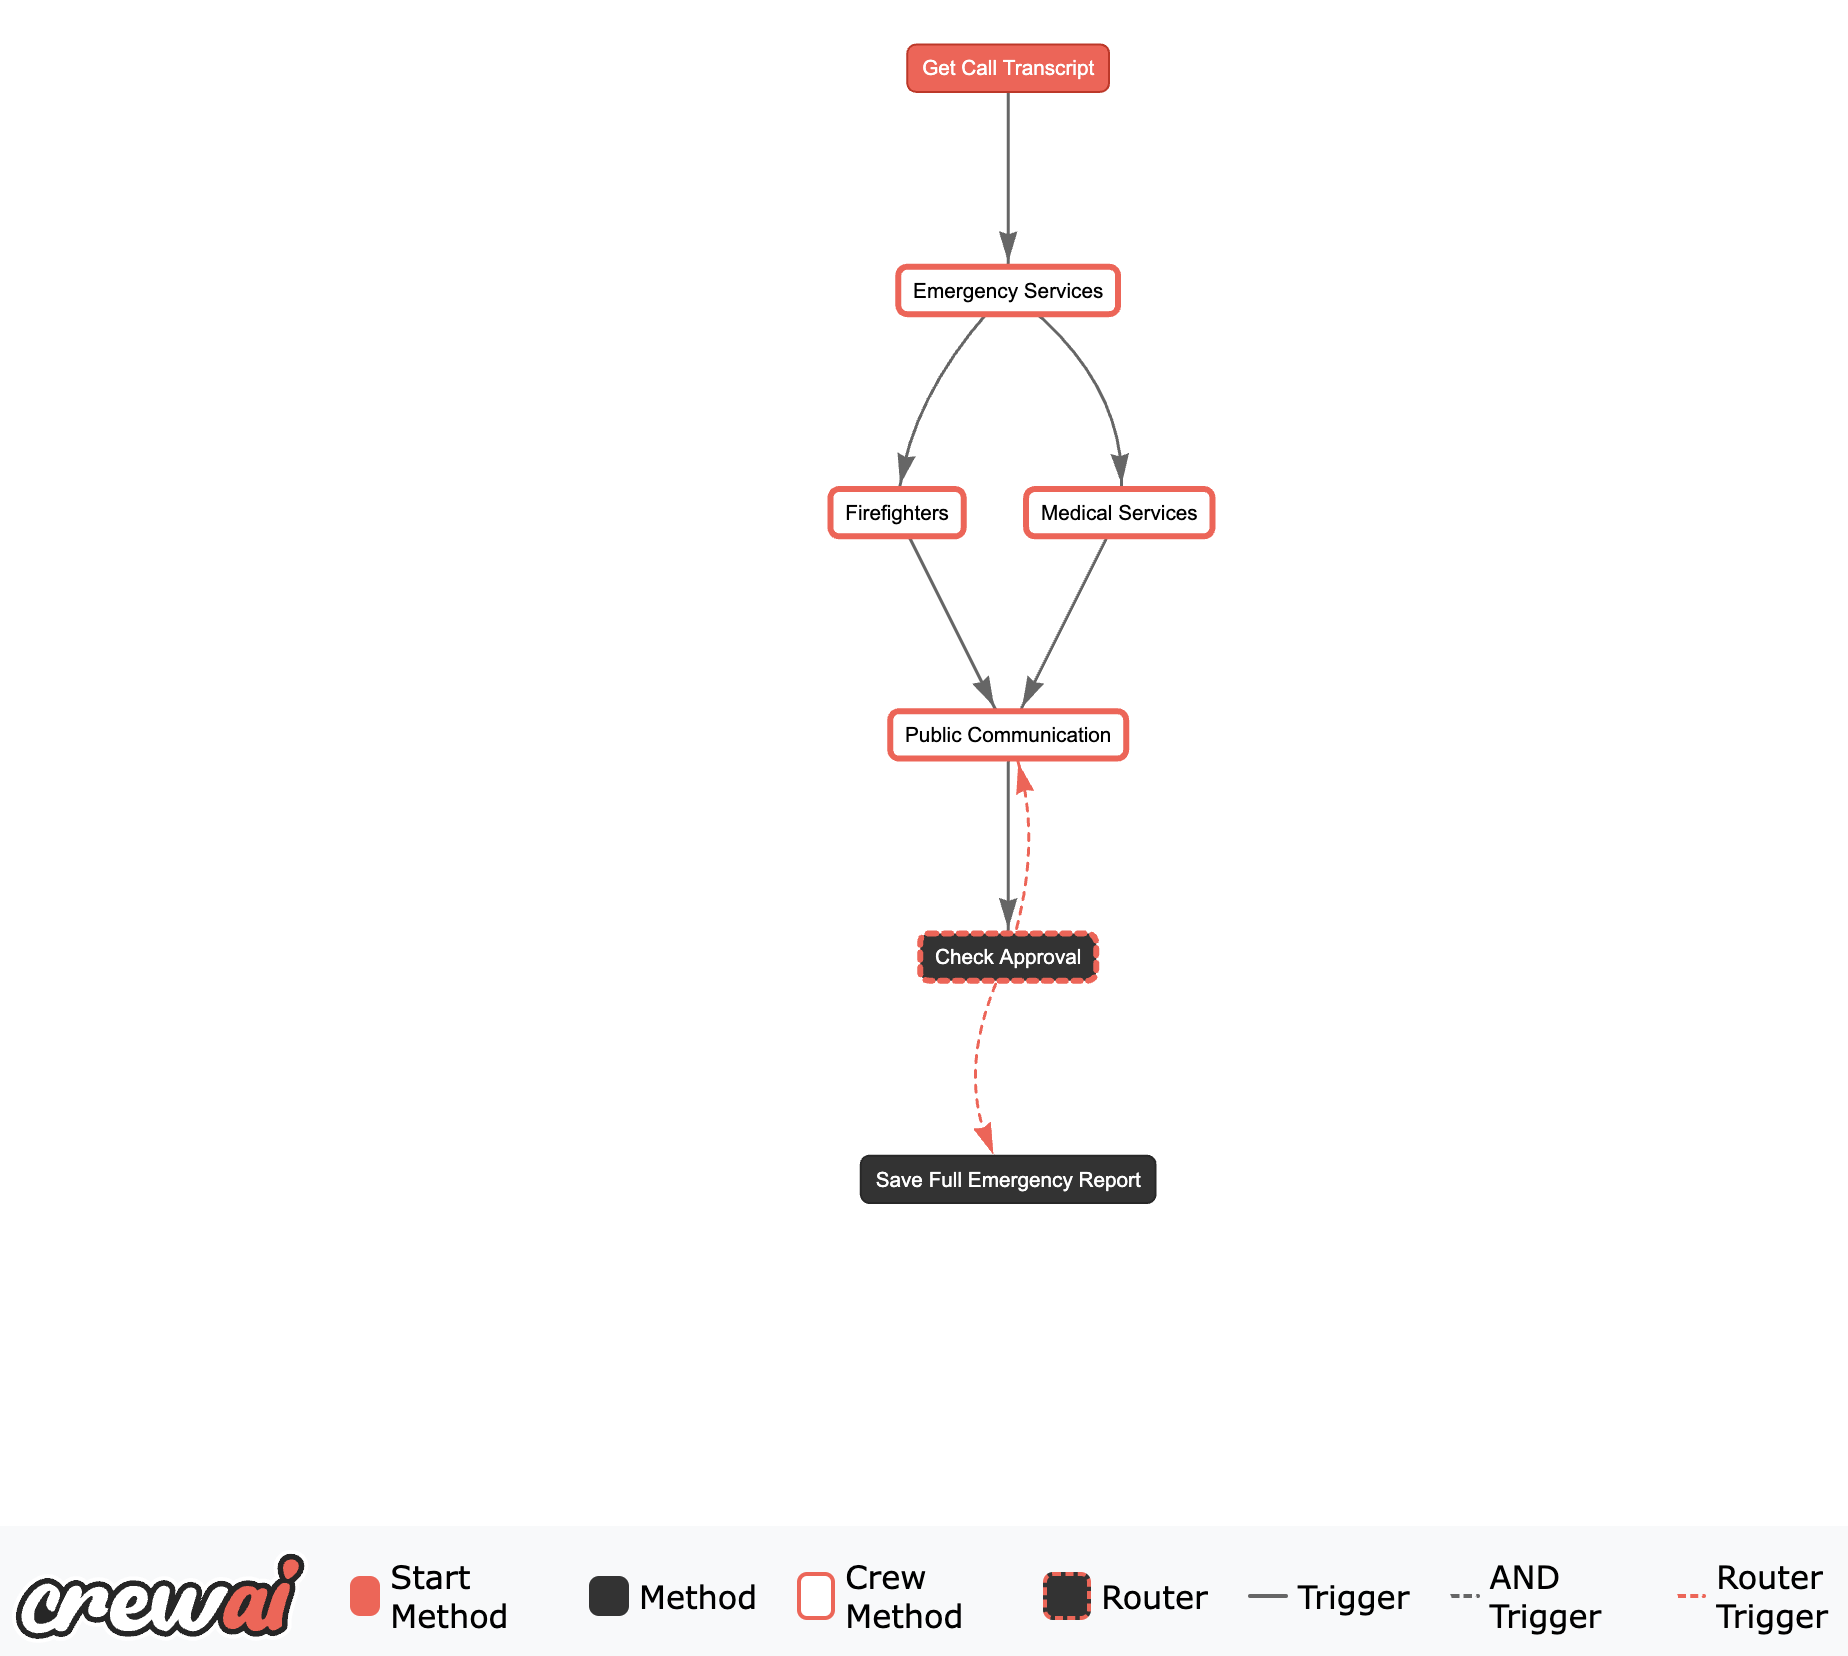
\includegraphics[width=0.8\textwidth]{figures/coordination_flow.png}
    \caption{Emergency Response Flow showing parallel processing paths and conditional triggers}
    \label{fig:interaction}
\end{figure}

As illustrated in Figure~\ref{fig:interaction}, the system uses logical operators (\texttt{and\_}, \texttt{or\_}) to create complex flow dependencies.

The flow is orchestrated using CrewAI's decorators, with complex triggering conditions:

\begin{lstlisting}[caption={Key Flow Control Points in Emergency Response}]
@start()
def get_call_transcript():
    # Initial entry point

@listen(get_call_transcript)
def emergency_services():
    # Processes emergency call

@listen(emergency_services)
def firefighters():
    # Parallel response team

@listen(emergency_services)
def medical_services():
    # Parallel response team

@listen(or_(and_(firefighters, medical_services), "retry public communication"))
def public_communication():
    # Activates after both teams report or during retries

@listen("save full emergency report")
def save_full_emergency_report():
    # Generates final report with all crew responses
\end{lstlisting}

\subsection{State Management}
The system maintains a centralized state using a Pydantic model that tracks all aspects of the emergency response:

\begin{lstlisting}[caption={Emergency Planner State Model}]
class EmergencyPlannerState(BaseModel):
    call_transcript: Optional[str]
    call_assessment: Optional[CallAssessment]
    firefighters_response_report: Optional[FirefightersResponseReport]
    medical_response_report: Optional[MedicalResponseReport]
    public_communication_report: Optional[PublicCommunicationReport]
    mayor_approval_retry_count: int = 0
\end{lstlisting}

This state model ensures:
\begin{itemize}
    \item Complete tracking of the emergency call lifecycle
    \item Type-safe storage of crew assessments and reports
    \item Monitoring of mayoral approval attempts
    \item Optional fields to accommodate partial state updates
\end{itemize}

In addition to basic state management, the flow also performs basic data transformations, such as deciding whether to activate the medical services crew based on the call assessment, and extracting relevant data to pass to subsequent crews.

\subsection{Router Implementation}
The system employs a router specifically for managing public communications:
\begin{lstlisting}[caption={Router Implementation for Public Communication Approval}]
@router(public_communication)
def check_approval():
    if public_communication_report.mayor_approved:
        return "save full emergency report"
    elif mayor_approval_retry_count >= MAX_MAYOR_APPROVAL_RETRY_COUNT:
        return "save full emergency report"
    mayor_approval_retry_count += 1
    return "retry public communication"
\end{lstlisting}

\subsection{Coordination Mechanism}
The system implements a message-passing protocol using CrewAI's flow decorators:
\begin{itemize}
    \item \texttt{@start()} marks the entry point for emergency call processing
    \item \texttt{@listen()} establishes dependencies between crew operations
    \item \texttt{@router()} handles conditional flow control
\end{itemize}

Parallel processing is achieved through independent \texttt{@listen} decorators, allowing medical and firefighter responses to operate concurrently. The flow concludes with a comprehensive emergency report that includes timestamps and summaries from all participating crews.